% Options for packages loaded elsewhere
\PassOptionsToPackage{unicode}{hyperref}
\PassOptionsToPackage{hyphens}{url}
\PassOptionsToPackage{dvipsnames,svgnames*,x11names*}{xcolor}
%
\documentclass[
]{krantz}
\usepackage{lmodern}
\usepackage{amssymb,amsmath}
\usepackage{ifxetex,ifluatex}
\ifnum 0\ifxetex 1\fi\ifluatex 1\fi=0 % if pdftex
  \usepackage[T1]{fontenc}
  \usepackage[utf8]{inputenc}
  \usepackage{textcomp} % provide euro and other symbols
\else % if luatex or xetex
  \usepackage{unicode-math}
  \defaultfontfeatures{Scale=MatchLowercase}
  \defaultfontfeatures[\rmfamily]{Ligatures=TeX,Scale=1}
\fi
% Use upquote if available, for straight quotes in verbatim environments
\IfFileExists{upquote.sty}{\usepackage{upquote}}{}
\IfFileExists{microtype.sty}{% use microtype if available
  \usepackage[]{microtype}
  \UseMicrotypeSet[protrusion]{basicmath} % disable protrusion for tt fonts
}{}
\makeatletter
\@ifundefined{KOMAClassName}{% if non-KOMA class
  \IfFileExists{parskip.sty}{%
    \usepackage{parskip}
  }{% else
    \setlength{\parindent}{0pt}
    \setlength{\parskip}{6pt plus 2pt minus 1pt}}
}{% if KOMA class
  \KOMAoptions{parskip=half}}
\makeatother
\usepackage{xcolor}
\IfFileExists{xurl.sty}{\usepackage{xurl}}{} % add URL line breaks if available
\IfFileExists{bookmark.sty}{\usepackage{bookmark}}{\usepackage{hyperref}}
\hypersetup{
  pdftitle={R and JavaScript},
  pdfauthor={John Coene},
  colorlinks=true,
  linkcolor=Maroon,
  filecolor=Maroon,
  citecolor=Blue,
  urlcolor=Blue,
  pdfcreator={LaTeX via pandoc}}
\urlstyle{same} % disable monospaced font for URLs
\usepackage{color}
\usepackage{fancyvrb}
\newcommand{\VerbBar}{|}
\newcommand{\VERB}{\Verb[commandchars=\\\{\}]}
\DefineVerbatimEnvironment{Highlighting}{Verbatim}{commandchars=\\\{\}}
% Add ',fontsize=\small' for more characters per line
\usepackage{framed}
\definecolor{shadecolor}{RGB}{248,248,248}
\newenvironment{Shaded}{\begin{snugshade}}{\end{snugshade}}
\newcommand{\AlertTok}[1]{\textcolor[rgb]{0.33,0.33,0.33}{#1}}
\newcommand{\AnnotationTok}[1]{\textcolor[rgb]{0.37,0.37,0.37}{\textbf{\textit{#1}}}}
\newcommand{\AttributeTok}[1]{\textcolor[rgb]{0.61,0.61,0.61}{#1}}
\newcommand{\BaseNTok}[1]{\textcolor[rgb]{0.06,0.06,0.06}{#1}}
\newcommand{\BuiltInTok}[1]{#1}
\newcommand{\CharTok}[1]{\textcolor[rgb]{0.5,0.5,0.5}{#1}}
\newcommand{\CommentTok}[1]{\textcolor[rgb]{0.37,0.37,0.37}{\textit{#1}}}
\newcommand{\CommentVarTok}[1]{\textcolor[rgb]{0.37,0.37,0.37}{\textbf{\textit{#1}}}}
\newcommand{\ConstantTok}[1]{\textcolor[rgb]{0,0,0}{#1}}
\newcommand{\ControlFlowTok}[1]{\textcolor[rgb]{0.27,0.27,0.27}{\textbf{#1}}}
\newcommand{\DataTypeTok}[1]{\textcolor[rgb]{0.27,0.27,0.27}{#1}}
\newcommand{\DecValTok}[1]{\textcolor[rgb]{0.06,0.06,0.06}{#1}}
\newcommand{\DocumentationTok}[1]{\textcolor[rgb]{0.37,0.37,0.37}{\textbf{\textit{#1}}}}
\newcommand{\ErrorTok}[1]{\textcolor[rgb]{0.14,0.14,0.14}{\textbf{#1}}}
\newcommand{\ExtensionTok}[1]{#1}
\newcommand{\FloatTok}[1]{\textcolor[rgb]{0.06,0.06,0.06}{#1}}
\newcommand{\FunctionTok}[1]{\textcolor[rgb]{0,0,0}{#1}}
\newcommand{\ImportTok}[1]{#1}
\newcommand{\InformationTok}[1]{\textcolor[rgb]{0.37,0.37,0.37}{\textbf{\textit{#1}}}}
\newcommand{\KeywordTok}[1]{\textcolor[rgb]{0.27,0.27,0.27}{\textbf{#1}}}
\newcommand{\NormalTok}[1]{#1}
\newcommand{\OperatorTok}[1]{\textcolor[rgb]{0.43,0.43,0.43}{\textbf{#1}}}
\newcommand{\OtherTok}[1]{\textcolor[rgb]{0.37,0.37,0.37}{#1}}
\newcommand{\PreprocessorTok}[1]{\textcolor[rgb]{0.37,0.37,0.37}{\textit{#1}}}
\newcommand{\RegionMarkerTok}[1]{#1}
\newcommand{\SpecialCharTok}[1]{\textcolor[rgb]{0,0,0}{#1}}
\newcommand{\SpecialStringTok}[1]{\textcolor[rgb]{0.5,0.5,0.5}{#1}}
\newcommand{\StringTok}[1]{\textcolor[rgb]{0.5,0.5,0.5}{#1}}
\newcommand{\VariableTok}[1]{\textcolor[rgb]{0,0,0}{#1}}
\newcommand{\VerbatimStringTok}[1]{\textcolor[rgb]{0.5,0.5,0.5}{#1}}
\newcommand{\WarningTok}[1]{\textcolor[rgb]{0.37,0.37,0.37}{\textbf{\textit{#1}}}}
\usepackage{longtable,booktabs}
% Correct order of tables after \paragraph or \subparagraph
\usepackage{etoolbox}
\makeatletter
\patchcmd\longtable{\par}{\if@noskipsec\mbox{}\fi\par}{}{}
\makeatother
% Allow footnotes in longtable head/foot
\IfFileExists{footnotehyper.sty}{\usepackage{footnotehyper}}{\usepackage{footnote}}
\makesavenoteenv{longtable}
\usepackage{graphicx,grffile}
\makeatletter
\def\maxwidth{\ifdim\Gin@nat@width>\linewidth\linewidth\else\Gin@nat@width\fi}
\def\maxheight{\ifdim\Gin@nat@height>\textheight\textheight\else\Gin@nat@height\fi}
\makeatother
% Scale images if necessary, so that they will not overflow the page
% margins by default, and it is still possible to overwrite the defaults
% using explicit options in \includegraphics[width, height, ...]{}
\setkeys{Gin}{width=\maxwidth,height=\maxheight,keepaspectratio}
% Set default figure placement to htbp
\makeatletter
\def\fps@figure{htbp}
\makeatother
\setlength{\emergencystretch}{3em} % prevent overfull lines
\providecommand{\tightlist}{%
  \setlength{\itemsep}{0pt}\setlength{\parskip}{0pt}}
\setcounter{secnumdepth}{5}
\usepackage{booktabs}
\usepackage{longtable}
\usepackage[bf,singlelinecheck=off]{caption}

\usepackage{framed,color}
\definecolor{shadecolor}{RGB}{248,248,248}

\renewcommand{\textfraction}{0.05}
\renewcommand{\topfraction}{0.8}
\renewcommand{\bottomfraction}{0.8}
\renewcommand{\floatpagefraction}{0.75}

\renewenvironment{quote}{\begin{VF}}{\end{VF}}
\let\oldhref\href
\renewcommand{\href}[2]{#2\footnote{\url{#1}}}

\makeatletter
\newenvironment{kframe}{%
\medskip{}
\setlength{\fboxsep}{.8em}
 \def\at@end@of@kframe{}%
 \ifinner\ifhmode%
  \def\at@end@of@kframe{\end{minipage}}%
  \begin{minipage}{\columnwidth}%
 \fi\fi%
 \def\FrameCommand##1{\hskip\@totalleftmargin \hskip-\fboxsep
 \colorbox{shadecolor}{##1}\hskip-\fboxsep
     % There is no \\@totalrightmargin, so:
     \hskip-\linewidth \hskip-\@totalleftmargin \hskip\columnwidth}%
 \MakeFramed {\advance\hsize-\width
   \@totalleftmargin\z@ \linewidth\hsize
   \@setminipage}}%
 {\par\unskip\endMakeFramed%
 \at@end@of@kframe}
\makeatother

\renewenvironment{Shaded}{\begin{kframe}}{\end{kframe}}

\usepackage{makeidx}
\makeindex

\urlstyle{tt}

\usepackage{amsthm}
\makeatletter
\def\thm@space@setup{%
  \thm@preskip=8pt plus 2pt minus 4pt
  \thm@postskip=\thm@preskip
}
\makeatother

\frontmatter
\usepackage{multicol}
\newcommand{\btwocol}{\begin{multicols}{2}}
\newcommand{\etwocol}{\end{multicols}}
\usepackage[]{natbib}
\bibliographystyle{apalike}

\title{R and JavaScript}
\author{John Coene}
\date{2020-01-22}

\begin{document}
\maketitle

% you may need to leave a few empty pages before the dedication page

%\cleardoublepage\newpage\thispagestyle{empty}\null
%\cleardoublepage\newpage\thispagestyle{empty}\null
%\cleardoublepage\newpage
\thispagestyle{empty}

\begin{center}
To my son,

without whom I should have finished this book two years earlier
%\includegraphics{images/dedication.pdf}
\end{center}

\setlength{\abovedisplayskip}{-5pt}
\setlength{\abovedisplayshortskip}{-5pt}

{
\hypersetup{linkcolor=}
\setcounter{tocdepth}{2}
\tableofcontents
}
\listoftables
\listoffigures
\hypertarget{preface}{%
\chapter*{Preface}\label{preface}}


The R programming language has seen the integration of many programming languages; C, C++, Python, to name a few, can be seamlessly embedded into R code. Little known to many, R works just as well with JavaScript---this book delves into the various ways both languages can work together.

The ultimate aim of this work is to put the reader at ease with inviting JavaScript in their data science workflow.

\hypertarget{about-the-author}{%
\chapter*{About the Author}\label{about-the-author}}


Frida Gomam is a famous lady. Police will always let her go.

\mainmatter

\hypertarget{intro}{%
\chapter{Introduction}\label{intro}}

In this chapter, after briefly going through prerequisites, we provide a rationale for integrating JavaScript with R which we support with examples, namely packages available on CRAN. Then, we list the various ways in which one might go about making both languages work together. Finally, we end with a review of concepts fundamental to fully understand the more advanced topics residing in later chapters.

\hypertarget{prerequisites}{%
\section*{Prerequisites}\label{prerequisites}}


The code contained in the following pages is approachable to readers with basic knowledge of R, although being familiar with \href{https://r6.r-lib.org/}{R6 classes} \citep{R-R6}, package development with \href{https://devtools.r-lib.org/}{devtools} \citep{R-devtools}, and \href{https://shiny.rstudio.com/}{Shiny} \citep{R-shiny} is helpful.

Only basic knowledge of JavaScript is required to understand and learn from the book as not only is JavaScript rather uncomplicated and its syntax similar to R's in places, we write surprisingly little of it. Understanding of JSON and HTML, however, is essential. In essence, if one has already used external JavaScript libraries in HTML or R markdown documents then one is well-equipped to tackle this book but in the event that you have not, we will go through a quick review of the basics of both JavaScript and JSON at the end of the chapter.

\hypertarget{rationale}{%
\section*{Rationale}\label{rationale}}


Why merge JavaScript and R? They are two fundamentally different languages that each have their strengths and weaknesses, combining the two allows making the most of their consolidated advantages and circumvent their respective limitations to produce software altogether better for it.

A fair reason to use JavaScript might simply be that the thing one wants to achieve in R has already been realised in JavaScript. Why reinvent the wheel when the solution already exists and that it can be made accessible from R? The R package \href{https://github.com/ropensci/lawn}{lawn} \citep{R-lawn} by Ropensci integrates \href{http://turfjs.org/}{turf.js}, a brilliant library for geo-spatial analysis. JavaScript is not required to make those computations, it could be rewritten solely in R but that would be vastly more laborious than wrapping the JavaScript API in R.

\begin{Shaded}
\begin{Highlighting}[]
\KeywordTok{library}\NormalTok{(lawn)}

\KeywordTok{lawn_count}\NormalTok{(lawn_data}\OperatorTok{$}\NormalTok{polygons_count, lawn_data}\OperatorTok{$}\NormalTok{points_count, }\StringTok{"population"}\NormalTok{)}
\end{Highlighting}
\end{Shaded}

\begin{verbatim}
## <FeatureCollection>
##   Bounding box: -112.1 46.6 -112.0 46.6
##   No. features: 2
##   No. points: 20
##   Properties: 
##     values count
## 1 200, 600     2
## 2              0
\end{verbatim}

Another great reason is that JavaScript can do things that R cannot, e.g.: run in the browser. Therefore one cannot natively create interactive visualisations with R. \href{https://plotly-r.com/}{Plotly} \citep{R-plotly} by Carson Sievert packages the \href{https://plot.ly/}{plotly JavaScript library} to let one create interactive visualisations solely from R code.

\begin{Shaded}
\begin{Highlighting}[]
\KeywordTok{library}\NormalTok{(plotly)}

\KeywordTok{plot_ly}\NormalTok{(diamonds, }\DataTypeTok{x =} \OperatorTok{~}\NormalTok{cut, }\DataTypeTok{color =} \OperatorTok{~}\NormalTok{clarity)}
\end{Highlighting}
\end{Shaded}

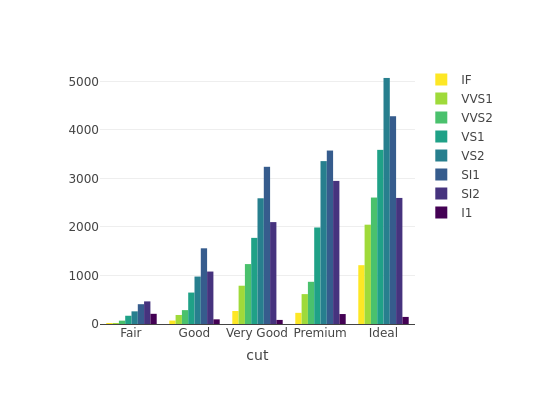
\includegraphics{bookdown_files/figure-latex/unnamed-chunk-2-1.png}

Finally, JavaScript can work together with R to improve how we communicate insights. One of the many ways in which Shiny stands out is that it lets one create web applications solely from R code with no knowledge of HTML, CSS, or JavaScript but that does not mean they can't extend Shiny, quite the contrary. The \href{http://waiter.john-coene.com/}{waiter package} \citep{R-waiter} integrates a variety of JavaScript libraries to display loading screens in Shiny applications.

\begin{Shaded}
\begin{Highlighting}[]
\KeywordTok{library}\NormalTok{(shiny)}
\KeywordTok{library}\NormalTok{(waiter)}

\NormalTok{ui <-}\StringTok{ }\KeywordTok{fluidPage}\NormalTok{(}
  \KeywordTok{use_waiter}\NormalTok{(), }\CommentTok{# include dependencies}
  \KeywordTok{actionButton}\NormalTok{(}\StringTok{"show"}\NormalTok{, }\StringTok{"Show loading for 3 seconds"}\NormalTok{)}
\NormalTok{)}

\NormalTok{server <-}\StringTok{ }\ControlFlowTok{function}\NormalTok{(input, output, session)\{}
  \CommentTok{# create a waiter}
\NormalTok{  w <-}\StringTok{ }\NormalTok{Waiter}\OperatorTok{$}\KeywordTok{new}\NormalTok{()}

  \CommentTok{# on button click}
  \KeywordTok{observeEvent}\NormalTok{(input}\OperatorTok{$}\NormalTok{show, \{}
\NormalTok{    w}\OperatorTok{$}\KeywordTok{show}\NormalTok{()}
    \KeywordTok{Sys.sleep}\NormalTok{(}\DecValTok{3}\NormalTok{)}
\NormalTok{    w}\OperatorTok{$}\KeywordTok{hide}\NormalTok{()}
\NormalTok{  \})}
\NormalTok{\}}

\KeywordTok{shinyApp}\NormalTok{(ui, server)}
\end{Highlighting}
\end{Shaded}

\begin{flushleft}
\includegraphics[width=6.25in]{images/waiter} \end{flushleft}

Hopefully this makes a couple of great reasons and alluring examples to entice you to persevere with this book.

\hypertarget{methods}{%
\section*{Methods}\label{methods}}


Though perhaps not obvious at first, all of the packages used as examples in the previous section internally interface with JavaScript very differently. As we'll discover, there many ways in which one can blend JavaScript with R, generally the way to go about it is dictated by the nature of is to be achieved.

Let's list the methods available to us to blend JavaScript with R before covering them each in-depth in their own respective chapter later in the book.

\hypertarget{v8}{%
\subsection*{V8}\label{v8}}


\href{https://github.com/jeroen/v8}{V8} by Jeroen Ooms is an R interface to Google's JavaScript engine. It will let you run JavaScript code directly from R and get the result back, it even comes with an interactive console. This is the way the lawn package used in a previous example has internally calls turf.js.

\begin{Shaded}
\begin{Highlighting}[]
\KeywordTok{library}\NormalTok{(V8)}

\NormalTok{ctx <-}\StringTok{ }\KeywordTok{v8}\NormalTok{()}

\NormalTok{ctx}\OperatorTok{$}\KeywordTok{eval}\NormalTok{(}\StringTok{"2 + 2"}\NormalTok{) }\CommentTok{# this is evaluated in JavaScript!}
\end{Highlighting}
\end{Shaded}

\begin{verbatim}
## [1] "4"
\end{verbatim}

\hypertarget{htmlwidgets}{%
\subsection*{htmlwidgets}\label{htmlwidgets}}


\href{http://www.htmlwidgets.org/}{htmlwidgets} \citep{R-htmlwidgets} specialises in wrapping JavaScript libraries that generate visual outputs. This is what packages such as plotly, \href{https://rstudio.github.io/DT/}{DT} \citep{R-DT}, \href{http://jkunst.com/highcharter/}{highcharter} \citep{R-highcharter}, and many more use to provide interactive visualisation with R.

It is by far the most popular integration out there, at the time of writing this it has been downloaded nearly 10 million times from CRAN. It will therefore be covered extensively in later chapters.

\hypertarget{shiny}{%
\subsection*{Shiny}\label{shiny}}


The Shiny framework allows creating applications accessible from web browsers where JavaScript natively runs, it follows that JavaScript can run \emph{alongside} such applications. Often overlooked though, the two can also work \emph{hand-in-hand} as one can pass data from the R server to the JavaScript front-end and vice versa. Some form of that tends to be included in htmlwidgets so one can pick up server-side which point on a scatter plot was clicked for instance.

\hypertarget{reactr}{%
\subsection*{reactR}\label{reactr}}


\href{https://react-r.github.io/reactR/}{ReactR} \citep{R-reactR} is an R package that emulates very well htmlwidgets but specifically for the \href{https://reactjs.org/}{React framework}. Unlike htmlwidgets it is not limited to visual outputs and also provides functions to build inputs, e.g.: a drop-down menu (like \texttt{shiny::selectInput}). The \href{https://glin.github.io/reactable/}{reactable package} \citep{R-reactable} uses reactR to enable building interactive tables solely from R code.

\begin{Shaded}
\begin{Highlighting}[]
\NormalTok{reactable}\OperatorTok{::}\KeywordTok{reactable}\NormalTok{(iris[}\DecValTok{1}\OperatorTok{:}\DecValTok{5}\NormalTok{, ], }\DataTypeTok{showPagination =} \OtherTok{TRUE}\NormalTok{)}
\end{Highlighting}
\end{Shaded}

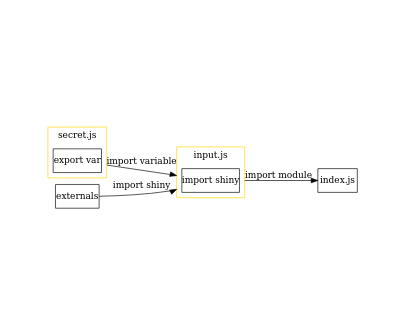
\includegraphics{bookdown_files/figure-latex/unnamed-chunk-4-1.png}

Note that custom Shiny inputs can also be built, this is however not covered in this book for it is very well \href{https://shiny.rstudio.com/articles/building-inputs.html}{documented}.

\hypertarget{bubble}{%
\subsection*{bubble}\label{bubble}}


\href{https://github.com/ColinFay/bubble}{bubble} \citep{R-bubble} by Colin Fay is a more recent R package, still under heady development but very promising: it lets one run \href{https://nodejs.org/en/}{node.js} code in R, comes with an interactive node REPL, the ability to install npm packages, and even an R markdown engine. It's similar to V8 in many ways.

\begin{Shaded}
\begin{Highlighting}[]
\KeywordTok{library}\NormalTok{(bubble)}

\NormalTok{n <-}\StringTok{ }\NormalTok{NodeSession}\OperatorTok{$}\KeywordTok{new}\NormalTok{() }

\NormalTok{n}\OperatorTok{$}\KeywordTok{eval}\NormalTok{(}\StringTok{"2 + 2"}\NormalTok{) }\CommentTok{# this is evaluated in node.js}
\end{Highlighting}
\end{Shaded}

\begin{verbatim}
## 4
\end{verbatim}

\hypertarget{r2d3}{%
\subsection*{r2d3}\label{r2d3}}


\href{https://rstudio.github.io/r2d3/}{r2d3} \citep{R-r2d3} by RStudio is an R package designed specifically to work with \href{https://d3js.org/}{d3.js}. It is similar to htmlwidgets but works rather differently.

\begin{Shaded}
\begin{Highlighting}[]
\CommentTok{# https://rstudio.github.io/r2d3/articles/gallery/chord/}
\NormalTok{r2d3}\OperatorTok{::}\KeywordTok{r2d3}\NormalTok{(}\DataTypeTok{data =} \KeywordTok{matrix}\NormalTok{(}\KeywordTok{round}\NormalTok{(}\KeywordTok{runif}\NormalTok{(}\DecValTok{16}\NormalTok{, }\DecValTok{1}\NormalTok{, }\DecValTok{10000}\NormalTok{)), }\DataTypeTok{ncol =} \DecValTok{4}\NormalTok{, }\DataTypeTok{nrow =} \DecValTok{4}\NormalTok{), }\DataTypeTok{script =} \StringTok{"chord.js"}\NormalTok{)}
\end{Highlighting}
\end{Shaded}

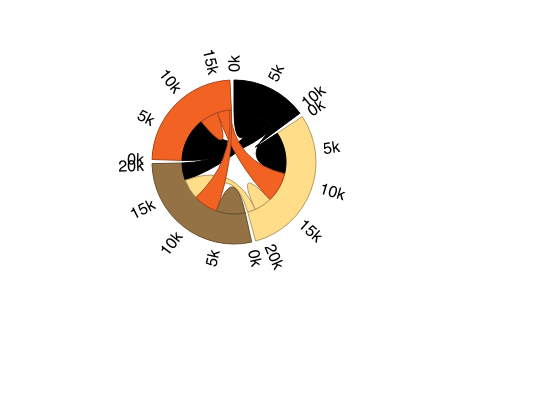
\includegraphics{bookdown_files/figure-latex/unnamed-chunk-6-1.png}

The packages bubble and V8 are intended for use of JavaScript for computations while r2d3, htmlwidgets, and reactR are designed to produce visual outputs (e.g.: graphs and tables), using JavaScript in Shiny can of course be used for the latter but is certainly not limited to that.

\hypertarget{json}{%
\section*{JSON}\label{json}}


JSON (JavaScript Object Notation) is a very popular data \emph{interchange} format with which we will work extensively throughout this book, it is thus crucial that we have a good understanding of it before we plunge into the nitty-gritty. As one might foresee, if we want two languages to work together it is essential that we have a data format that can be understood by both---JSON lets us harmoniously pass data from one to the other. While it is natively supported in JavaScript, it can be graciously handled in R with the \href{https://CRAN.R-project.org/package=jsonlite}{jsonlite package} \citep{R-jsonlite}, in fact it is the serialiser used internally by all of the methods detailed in the previous section.

JSON is to all intents and purposes the equivalent of lists in R; a flexible data format that can store pretty much anything. Below we create a nested list and convert it to JSON with the help of jsonlite, we set \texttt{pretty} to \texttt{TRUE} to add indentation for clearer printing.

\begin{Shaded}
\begin{Highlighting}[]
\CommentTok{# install.packages("jsonlite")}
\KeywordTok{library}\NormalTok{(jsonlite)}

\NormalTok{lst <-}\StringTok{ }\KeywordTok{list}\NormalTok{(}
  \DataTypeTok{a =} \DecValTok{1}\NormalTok{,}
  \DataTypeTok{b =} \KeywordTok{list}\NormalTok{(}
    \DataTypeTok{c =} \KeywordTok{c}\NormalTok{(}\StringTok{"A"}\NormalTok{, }\StringTok{"B"}\NormalTok{)}
\NormalTok{  ),}
  \DataTypeTok{d =} \DecValTok{1}\OperatorTok{:}\DecValTok{5}
\NormalTok{)}

\KeywordTok{toJSON}\NormalTok{(lst, }\DataTypeTok{pretty =} \OtherTok{TRUE}\NormalTok{)}
\end{Highlighting}
\end{Shaded}

\begin{verbatim}
## {
##   "a": [1],
##   "b": {
##     "c": ["A", "B"]
##   },
##   "d": [1, 2, 3, 4, 5]
## }
\end{verbatim}

Looking closely at the list and JSON output above one quickly sees the resemblance. Something seems odd though, the first value in the list (\texttt{a\ =\ 1}) was serialised; to an array (vector) of length one (\texttt{"a":\ {[}1{]}}) where would probably expect an integer instead. This is not a mistake, we often forget that there are no scalar types in R and that \texttt{a} is in fact a vector as we can observe below.

\begin{Shaded}
\begin{Highlighting}[]
\NormalTok{x <-}\StringTok{ }\DecValTok{1}
\KeywordTok{is.vector}\NormalTok{(x)}
\end{Highlighting}
\end{Shaded}

\begin{verbatim}
## [1] TRUE
\end{verbatim}

JavaScript, on the other hand, does have scalar types, more often than not we will want to convert our vectors of length one to scalar types rather than arrays of length one. To do so we need use the \texttt{auto\_unbox} argument in \texttt{jsonlite::toJSON}, we'll do this most of the time we have to convert data to JSON.

\begin{Shaded}
\begin{Highlighting}[]
\KeywordTok{toJSON}\NormalTok{(lst, }\DataTypeTok{pretty =} \OtherTok{TRUE}\NormalTok{, }\DataTypeTok{auto_unbox =} \OtherTok{TRUE}\NormalTok{)}
\end{Highlighting}
\end{Shaded}

\begin{verbatim}
## {
##   "a": 1,
##   "b": {
##     "c": ["A", "B"]
##   },
##   "d": [1, 2, 3, 4, 5]
## }
\end{verbatim}

As demonstrated above the vector of length one was ``unboxed'' into an integer, with \texttt{auto\_unbox} set to \texttt{TRUE} jsonlite will properly convert such vectors into their appropriate type; integer, numeric, boolean, etc. If JSON is more or less the equivalent of lists in R one might wonder how jsonlite handles data frames.

\begin{Shaded}
\begin{Highlighting}[]
\CommentTok{# subset of built-in dataset}
\NormalTok{df <-}\StringTok{ }\NormalTok{cars[}\DecValTok{1}\OperatorTok{:}\DecValTok{2}\NormalTok{, ]}

\KeywordTok{toJSON}\NormalTok{(df, }\DataTypeTok{pretty =} \OtherTok{TRUE}\NormalTok{)}
\end{Highlighting}
\end{Shaded}

\begin{verbatim}
## [
##   {
##     "speed": 4,
##     "dist": 2
##   },
##   {
##     "speed": 4,
##     "dist": 10
##   }
## ]
\end{verbatim}

What jsonlite does internally is essentially turn the data.frame into a list \emph{rowwise} to produce a list for every row. This generally how rectangular data is represented in lists, for instance, \texttt{purrr::transpose} does the same. We can reproduce this with the snippet below, we remove row names and use apply to turn every row into a list.

\begin{Shaded}
\begin{Highlighting}[]
\KeywordTok{row.names}\NormalTok{(df) <-}\StringTok{ }\OtherTok{NULL}
\NormalTok{df_list <-}\StringTok{ }\KeywordTok{apply}\NormalTok{(df, }\DecValTok{1}\NormalTok{, as.list)}

\KeywordTok{toJSON}\NormalTok{(df_list, }\DataTypeTok{pretty =} \OtherTok{TRUE}\NormalTok{, }\DataTypeTok{auto_unbox =} \OtherTok{TRUE}\NormalTok{)}
\end{Highlighting}
\end{Shaded}

\begin{verbatim}
## [
##   {
##     "speed": 4,
##     "dist": 2
##   },
##   {
##     "speed": 4,
##     "dist": 10
##   }
## ]
\end{verbatim}

Jsonlite of course also enables reading data from JSON into R with the function \texttt{fromJSON}.

\begin{Shaded}
\begin{Highlighting}[]
\NormalTok{json <-}\StringTok{ }\KeywordTok{toJSON}\NormalTok{(df) }\CommentTok{# convert to JSON}
\KeywordTok{fromJSON}\NormalTok{(json) }\CommentTok{# read from JSON}
\end{Highlighting}
\end{Shaded}

\begin{verbatim}
##   speed dist
## 1     4    2
## 2     4   10
\end{verbatim}

It's important to note that jsonlite did the conversion back to a data frame. Therefore the code below also returns a data frame even though the object we initially converted to JSON is a list.

\begin{Shaded}
\begin{Highlighting}[]
\KeywordTok{class}\NormalTok{(df_list)}
\end{Highlighting}
\end{Shaded}

\begin{verbatim}
## [1] "list"
\end{verbatim}

\begin{Shaded}
\begin{Highlighting}[]
\NormalTok{json <-}\StringTok{ }\KeywordTok{toJSON}\NormalTok{(df_list)}
\KeywordTok{fromJSON}\NormalTok{(json)}
\end{Highlighting}
\end{Shaded}

\begin{verbatim}
##   speed dist
## 1     4    2
## 2     4   10
\end{verbatim}

Jsonlite provides many more options and functions that will let you tune JSON data in read to and written from R. Also, the jsonlite package does far more than what we detailed but at this juncture this is an adequate understanding of things.

\hypertarget{javascript}{%
\section*{JavaScript}\label{javascript}}


The book is not meant to teach one JavaScript, only to show how graciously it can work with R; in that endeavour we aim at writing little JavaScript so the book remains approachable to a wide audience. Let us just go through the very basics to ensure we know enough to get started with the next chapter.

In the event that you would want to try what we briefly explore here: the easiest way is to create an HTML file, write your code within a script tag and open the file in your web browser. The output can be observed in the console of the browser which can be opened with a right click and selecting ``inspect'' then going to the ``console'' tab.

\begin{Shaded}
\begin{Highlighting}[]
 \ErrorTok{<}\NormalTok{!–– index.html ––>}
\KeywordTok{<html>}
  \KeywordTok{<head>}
  \KeywordTok{</head>}
  \KeywordTok{<body>}
    \KeywordTok{<p}\OtherTok{ id=}\StringTok{"content"}\KeywordTok{>}\NormalTok{Trying JavaScript!}\KeywordTok{</p>}
  \KeywordTok{</body>}
  \KeywordTok{<script>}
    \CommentTok{// place your JavaScript code here}
  \KeywordTok{</script>}
\KeywordTok{</html>}
\end{Highlighting}
\end{Shaded}

The first difference with R is that the end of every line should be marked with a semi-colon. JavaScript code will often work without but one should always include them to avoid issues. Below we use \texttt{console.log}, JavaScript equivalent of R's \texttt{print} function.

\begin{Shaded}
\begin{Highlighting}[]
\VariableTok{console}\NormalTok{.}\AttributeTok{log}\NormalTok{(}\StringTok{"hello JavaScript"}\NormalTok{) }\CommentTok{// bad}
\VariableTok{console}\NormalTok{.}\AttributeTok{log}\NormalTok{(}\StringTok{"hello JavaScript"}\NormalTok{)}\OperatorTok{;} \CommentTok{// good}
\end{Highlighting}
\end{Shaded}

Another difference is that variables must be declared with keywords such as \texttt{var} or \texttt{const} to declare a constant.

\begin{Shaded}
\begin{Highlighting}[]
\NormalTok{x }\OperatorTok{=} \DecValTok{1}\OperatorTok{;} \CommentTok{// bad}
\KeywordTok{var}\NormalTok{ x }\OperatorTok{=} \DecValTok{1}\OperatorTok{;} \CommentTok{// good}
\end{Highlighting}
\end{Shaded}

One can declare a variable without assigning a value to it, to then do so later on.

\begin{Shaded}
\begin{Highlighting}[]
\CommentTok{// good}
\KeywordTok{var}\NormalTok{ y}\OperatorTok{;} 
\NormalTok{y }\OperatorTok{=}\NormalTok{ [}\DecValTok{1}\OperatorTok{,}\DecValTok{2}\OperatorTok{,}\DecValTok{3}\NormalTok{]}\OperatorTok{;}
\end{Highlighting}
\end{Shaded}

In R like in JavaScript, variables can be accessed from the parent environment (often referred to as ``context'' in the latter). One immense difference though is that while it is seen as bad practice in R it is not in JavaScript where it comes very useful.

\begin{Shaded}
\begin{Highlighting}[]
\CommentTok{# it works but don't do this}
\NormalTok{x <-}\StringTok{ }\DecValTok{123}
\NormalTok{foo <-}\StringTok{ }\ControlFlowTok{function}\NormalTok{()\{}
  \KeywordTok{print}\NormalTok{(x)}
\NormalTok{\}}
\KeywordTok{foo}\NormalTok{()}
\end{Highlighting}
\end{Shaded}

\begin{verbatim}
## [1] 123
\end{verbatim}

The above R code can be re-written in JavaScript. Note the slight variation in the function declaration.

\begin{Shaded}
\begin{Highlighting}[]
\CommentTok{// this is perfectly fine}
\KeywordTok{var}\NormalTok{ x }\OperatorTok{=} \DecValTok{1}\OperatorTok{;}

\KeywordTok{function} \AttributeTok{foo}\NormalTok{()}\OperatorTok{\{}
  \VariableTok{console}\NormalTok{.}\AttributeTok{log}\NormalTok{(x)}\OperatorTok{;} 
\OperatorTok{\}}

\AttributeTok{foo}\NormalTok{()}
\end{Highlighting}
\end{Shaded}

One concept which does not exist in R is that of the ``DOM'' which stands for Document Object Model. When a web page is loaded, the browser creates a Document Object Model of the page which can be accessed in JavaScript from the \texttt{document} object. This lets the developer programmatically manipulate the page itself so one can for instance, remove a button, change the text of an element, and plenty more.

The JavaScript code below grabs the element where \texttt{id=content} from the \texttt{document} with \texttt{getElementById}.

\begin{Shaded}
\begin{Highlighting}[]
 \ErrorTok{<}\NormalTok{!–– index.html ––>}
\KeywordTok{<html>}
  \KeywordTok{<head>}
  \KeywordTok{</head>}
  \KeywordTok{<body>}
    \KeywordTok{<p}\OtherTok{ id=}\StringTok{"content"}\KeywordTok{>}\NormalTok{Trying JavaScript!}\KeywordTok{</p>}
  \KeywordTok{</body>}
  \KeywordTok{<script>}
    \KeywordTok{var}\NormalTok{ cnt }\OperatorTok{=} \VariableTok{document}\NormalTok{.}\AttributeTok{getElementById}\NormalTok{(}\StringTok{"content"}\NormalTok{)}\OperatorTok{;}
    \VariableTok{cnt}\NormalTok{.}\AttributeTok{innerText} \OperatorTok{=} \StringTok{"The text has changed"}\OperatorTok{;}
  \KeywordTok{</script>}
\KeywordTok{</html>}
\end{Highlighting}
\end{Shaded}

This of course only scratched the surface of JavaScript but provides ample understanding of the language to go ahead with the rest of the book.

\hypertarget{the-v8-engine}{%
\chapter{The V8 Engine}\label{the-v8-engine}}

V8 is an R interface to Google's open source JavaScript engine of the same name, it powers Google Chrome, node.js and many other things. It is the first integration of JavaScript with R that we cover in this book. Both the V8 package and the engine it wraps are simple yet amazingly powerful.

\hypertarget{installation}{%
\section*{Installation}\label{installation}}


First install the V8 engine itself, instructions to do so are well detailed on \href{https://github.com/jeroen/v8\#installation}{V8's README} and below.

On Debian or Ubuntu use the code below from the terminal to install \href{https://v8.dev/}{libv8}.

\begin{Shaded}
\begin{Highlighting}[]
\FunctionTok{sudo}\NormalTok{ apt-get install -y libv8-dev}
\end{Highlighting}
\end{Shaded}

On Centos install v8-devel, which requires the EPEL tools.

\begin{Shaded}
\begin{Highlighting}[]
\FunctionTok{sudo}\NormalTok{ yum install epel-release}
\FunctionTok{sudo}\NormalTok{ yum install v8-devel}
\end{Highlighting}
\end{Shaded}

On Mac OS use \href{https://brew.sh/}{Homebrew}.

\begin{Shaded}
\begin{Highlighting}[]
\ExtensionTok{brew}\NormalTok{ install v8}
\end{Highlighting}
\end{Shaded}

Then install the R package from CRAN.

\begin{Shaded}
\begin{Highlighting}[]
\KeywordTok{install.packages}\NormalTok{(}\StringTok{"V8"}\NormalTok{)}
\end{Highlighting}
\end{Shaded}

\hypertarget{basics}{%
\section*{Basics}\label{basics}}


V8 provides a reference class, which pertains to object-oriented programming, hence it might look unconventional to many R users. It's nonetheless easy to grasp. If one wants to learn more about the R6's reference class system Hadley Wickham has a very good chapter on it in his \href{https://adv-r.hadley.nz/r6.html}{Advanced R} book.

Let's explore the basic functionalities of the package. First, load the library and use the function \texttt{v8} to instantiate a class.

\begin{Shaded}
\begin{Highlighting}[]
\KeywordTok{library}\NormalTok{(V8)}

\NormalTok{engine <-}\StringTok{ }\KeywordTok{v8}\NormalTok{()}
\end{Highlighting}
\end{Shaded}

The \texttt{eval} method allows running JavaScript code from R and retrive the results.

\begin{Shaded}
\begin{Highlighting}[]
\NormalTok{engine}\OperatorTok{$}\KeywordTok{eval}\NormalTok{(}\StringTok{"var x = 3 + 4;"}\NormalTok{) }\CommentTok{# this is evealuated in R}
\NormalTok{engine}\OperatorTok{$}\KeywordTok{eval}\NormalTok{(}\StringTok{"x"}\NormalTok{)}
\end{Highlighting}
\end{Shaded}

\begin{verbatim}
## [1] "7"
\end{verbatim}

Two observations on the above snippet of code. First, the variable we got back in R is a character vector when it should have been either an integer or a numeric. This is because we used the \texttt{eval} method which merely prints the output, \texttt{get} is more appropriate; it converts it to an appropriate R equivalent.

\begin{Shaded}
\begin{Highlighting}[]
\CommentTok{# retrieve our previously created variable}
\NormalTok{(x <-}\StringTok{ }\NormalTok{engine}\OperatorTok{$}\KeywordTok{get}\NormalTok{(}\StringTok{"x"}\NormalTok{))}
\end{Highlighting}
\end{Shaded}

\begin{verbatim}
## [1] 7
\end{verbatim}

\begin{Shaded}
\begin{Highlighting}[]
\KeywordTok{class}\NormalTok{(x)}
\end{Highlighting}
\end{Shaded}

\begin{verbatim}
## [1] "integer"
\end{verbatim}

Second, while creating a scalar with \texttt{eval("var\ x\ =\ 1;")} appears painless, imagine if you will the horror of having to convert a data frame to a JavaScript array via jsonlite then flatten it to character string so it can be used with the \texttt{eval} method. Horrid. Thankfully V8 comes with a method \texttt{assign}, complimentary to \texttt{get}, which declares R objects as JavaScript variables. It takes two arguments, first the name of the variable to create, second the object to assign to it.

\begin{Shaded}
\begin{Highlighting}[]
\CommentTok{# assign and retrieve a data.frame}
\NormalTok{engine}\OperatorTok{$}\KeywordTok{assign}\NormalTok{(}\StringTok{"vehicles"}\NormalTok{, cars[}\DecValTok{1}\OperatorTok{:}\DecValTok{3}\NormalTok{, ])}
\NormalTok{engine}\OperatorTok{$}\KeywordTok{get}\NormalTok{(}\StringTok{"vehicles"}\NormalTok{)}
\end{Highlighting}
\end{Shaded}

\begin{verbatim}
##   speed dist
## 1     4    2
## 2     4   10
## 3     7    4
\end{verbatim}

All of the conversion is handled by V8 internally with jsonlite as demonstrated in the previous chapter. We can confirm that the data frame was converted to a list rowwise; using \texttt{JSON.stringify} to display how the object is store in V8.

\begin{Shaded}
\begin{Highlighting}[]
\KeywordTok{cat}\NormalTok{(engine}\OperatorTok{$}\KeywordTok{eval}\NormalTok{(}\StringTok{"JSON.stringify(vehicles, null, 2);"}\NormalTok{))}
\end{Highlighting}
\end{Shaded}

\begin{verbatim}
## [
##   {
##     "speed": 4,
##     "dist": 2
##   },
##   {
##     "speed": 4,
##     "dist": 10
##   },
##   {
##     "speed": 7,
##     "dist": 4
##   }
## ]
\end{verbatim}

However the cyclical loop of 1) creating a variable in JavaScript to 2) run a function on the aforementioned object 3) get the results back in R, can be tedious. So V8 also allows calling JavaScript functions on R objects directly with the \texttt{call} method and obtain the results back in R.

\begin{Shaded}
\begin{Highlighting}[]
\NormalTok{engine}\OperatorTok{$}\KeywordTok{eval}\NormalTok{(}\StringTok{"new Date();"}\NormalTok{) }\CommentTok{# using eval}
\end{Highlighting}
\end{Shaded}

\begin{verbatim}
## [1] "Wed Jan 22 2020 21:56:51 GMT+0100 (CET)"
\end{verbatim}

\begin{Shaded}
\begin{Highlighting}[]
\NormalTok{engine}\OperatorTok{$}\KeywordTok{call}\NormalTok{(}\StringTok{"Date"}\NormalTok{, }\KeywordTok{Sys.Date}\NormalTok{()) }\CommentTok{# using call}
\end{Highlighting}
\end{Shaded}

\begin{verbatim}
## [1] "Wed Jan 22 2020 21:56:51 GMT+0100 (CET)"
\end{verbatim}

Finally, one can run code interactively rather than as strings by calling the console from the engine with \texttt{engine\$console()} you can then exit the console by typing \texttt{exit} or hitting the ESC key.

\hypertarget{external-libraries}{%
\section*{External Libraries}\label{external-libraries}}


V8 is actually quite bare in and of itself, there is for instance no functionalities built-in to read or write files from disk, it thus becomes truly interesting when you can use it JavaScript libraries. We do so with the \texttt{source} method which takes a \texttt{file} argument that will accept a path or URL to a JavaScript file to source. We'll demonstrate this using \href{https://fusejs.io/}{fuse.js} a fuzzy-search library.

\begin{Shaded}
\begin{Highlighting}[]
\NormalTok{engine}\OperatorTok{$}\KeywordTok{source}\NormalTok{(}\StringTok{"https://cdnjs.cloudflare.com/ajax/libs/fuse.js/3.4.6/fuse.min.js"}\NormalTok{)}
\end{Highlighting}
\end{Shaded}

\begin{verbatim}
## [1] "true"
\end{verbatim}

You can think of it as using the \texttt{script} tag in HTML to source (\texttt{src}) said file from disk or CDN.

\begin{Shaded}
\begin{Highlighting}[]
\KeywordTok{<html>}
  \KeywordTok{<head>}
    \KeywordTok{<script}\OtherTok{ src=}\StringTok{'https://cdnjs.cloudflare.com/ajax/libs/fuse.js/3.4.6/fuse.min.js'}\KeywordTok{></script>}
  \KeywordTok{</head>}
  \KeywordTok{<body>}
    \KeywordTok{<p>}\NormalTok{Content}\KeywordTok{</p>}
  \KeywordTok{</body>}
\KeywordTok{</html>}
\end{Highlighting}
\end{Shaded}

With the library imported we can use its functionalities. We'll replicate an example from fuse.js official website where it executes a search on an object that contains books and looks like JSON below.

\begin{Shaded}
\begin{Highlighting}[]
\KeywordTok{var}\NormalTok{ books }\OperatorTok{=}\NormalTok{ [}\OperatorTok{\{}
  \StringTok{'ISBN'}\OperatorTok{:} \StringTok{'A'}\OperatorTok{,}
  \StringTok{'title'}\OperatorTok{:} \StringTok{"Old Man's War"}\OperatorTok{,}
  \StringTok{'author'}\OperatorTok{:} \StringTok{'John Scalzi'}
\OperatorTok{\},} \OperatorTok{\{}
  \StringTok{'ISBN'}\OperatorTok{:} \StringTok{'B'}\OperatorTok{,}
  \StringTok{'title'}\OperatorTok{:} \StringTok{'The Lock Artist'}\OperatorTok{,}
  \StringTok{'author'}\OperatorTok{:} \StringTok{'Steve Hamilton'}
\OperatorTok{\}}\NormalTok{]}
\end{Highlighting}
\end{Shaded}

This can be easily created, as we've already seen this is just how V8 creates data frames. We define a data.frame of books that looks similar and load it into our engine.

\begin{Shaded}
\begin{Highlighting}[]
\NormalTok{books <-}\StringTok{ }\KeywordTok{data.frame}\NormalTok{(}
  \DataTypeTok{title =} \KeywordTok{c}\NormalTok{(}
    \StringTok{"Rights of Man"}\NormalTok{,}
    \StringTok{"Black Swan"}\NormalTok{,}
    \StringTok{"Common Sense"}\NormalTok{,}
    \StringTok{"Sense and Sensibility"}
\NormalTok{  ),}
  \DataTypeTok{id =} \KeywordTok{c}\NormalTok{(}\StringTok{"a"}\NormalTok{, }\StringTok{"b"}\NormalTok{, }\StringTok{"c"}\NormalTok{, }\StringTok{"d"}\NormalTok{)}
\NormalTok{)}

\NormalTok{engine}\OperatorTok{$}\KeywordTok{assign}\NormalTok{(}\StringTok{"books"}\NormalTok{, books)}
\end{Highlighting}
\end{Shaded}

Then again we can make sure that the data.frame was turned into a rowwise JSON object.

\begin{Shaded}
\begin{Highlighting}[]
\KeywordTok{cat}\NormalTok{(engine}\OperatorTok{$}\KeywordTok{eval}\NormalTok{(}\StringTok{"JSON.stringify(books, null, 2);"}\NormalTok{))}
\end{Highlighting}
\end{Shaded}

\begin{verbatim}
## [
##   {
##     "title": "Rights of Man",
##     "id": "a"
##   },
##   {
##     "title": "Black Swan",
##     "id": "b"
##   },
##   {
##     "title": "Common Sense",
##     "id": "c"
##   },
##   {
##     "title": "Sense and Sensibility",
##     "id": "d"
##   }
## ]
\end{verbatim}

Now we can define options for our search, we don't get into the details of fuse.js here as this is not the purpose of this book, you can read more about the options in the \href{https://fusejs.io/\#Examples}{examples section} of the site. We can mimic the format of the JSON options shown on the website with a simple list and assign that to our engine. If this confuses read the \href{intro.html\#json}{JSON section of the introduction}.

\btwocol

\begin{Shaded}
\begin{Highlighting}[]
\CommentTok{// JavaScript}
\KeywordTok{var}\NormalTok{ options }\OperatorTok{=} \OperatorTok{\{}
  \DataTypeTok{keys}\OperatorTok{:}\NormalTok{ [}\StringTok{'title'}\NormalTok{]}\OperatorTok{,}
  \DataTypeTok{id}\OperatorTok{:} \StringTok{'id'}
\OperatorTok{\}}
\end{Highlighting}
\end{Shaded}

\etwocol

\begin{Shaded}
\begin{Highlighting}[]
\CommentTok{# R}
\NormalTok{options <-}\StringTok{ }\KeywordTok{list}\NormalTok{(}
  \DataTypeTok{keys =} \KeywordTok{list}\NormalTok{(}\StringTok{"title"}\NormalTok{),}
  \DataTypeTok{id =} \StringTok{"id"}
\NormalTok{)}

\NormalTok{engine}\OperatorTok{$}\KeywordTok{assign}\NormalTok{(}\StringTok{"options"}\NormalTok{, options)}
\end{Highlighting}
\end{Shaded}

Then we can finish the second step of the online examples, instantiate a fuse.js object with our books and options objects then make a simple search, we assign the results of the search to an object which we then retrieve in R with \texttt{get}.

\begin{Shaded}
\begin{Highlighting}[]
\NormalTok{engine}\OperatorTok{$}\KeywordTok{eval}\NormalTok{(}\StringTok{"var fuse = new Fuse(books, options)"}\NormalTok{)}
\NormalTok{engine}\OperatorTok{$}\KeywordTok{eval}\NormalTok{(}\StringTok{"var results = fuse.search('sense')"}\NormalTok{)}
\NormalTok{engine}\OperatorTok{$}\KeywordTok{get}\NormalTok{(}\StringTok{"results"}\NormalTok{)}
\end{Highlighting}
\end{Shaded}

\begin{verbatim}
## [1] "d" "c"
\end{verbatim}

A search for ``sense'' returns a vector of ids where the term ``sense'' was found; \texttt{c} and \texttt{d} or the books Common Sense, Sense and Sensibility. We could perhaps make that last code simpler using the \texttt{call} method.

\begin{Shaded}
\begin{Highlighting}[]
\NormalTok{engine}\OperatorTok{$}\KeywordTok{call}\NormalTok{(}\StringTok{"fuse.search"}\NormalTok{, }\StringTok{"sense"}\NormalTok{)}
\end{Highlighting}
\end{Shaded}

\begin{verbatim}
## [1] "d" "c"
\end{verbatim}

\hypertarget{with-npm}{%
\section*{With Npm}\label{with-npm}}


We can also use \href{https://www.npmjs.com/}{npm} packages, though not all will work. Npm is Node's Package Manager, or in a sense Node's equivalent of CRAN.

To use npm packages we need \href{http://browserify.org/}{browserify}, a node library to bundle all dependencies of an npm package into a single, file which we can subsequently source in V8. Browserify is itself an npm package and there requires node and npm installed.

You can install browserify globally with the following command from the terminal.

\begin{Shaded}
\begin{Highlighting}[]
\ExtensionTok{npm}\NormalTok{ install -g browserify}
\end{Highlighting}
\end{Shaded}

We can now browserify an npm package. To demonstrate we will use \href{https://github.com/zeit/ms}{ms} which converts various time formats to milliseconds. First we install the package.

\begin{Shaded}
\begin{Highlighting}[]
\ExtensionTok{npm}\NormalTok{ install ms}
\end{Highlighting}
\end{Shaded}

Then we browserify it. The first line creates a file called \texttt{in.js} which contains \texttt{global.ms\ =\ require(\textquotesingle{}ms\textquotesingle{});} we then call browserify on that file specifying \texttt{ms.js} as output file.

\begin{Shaded}
\begin{Highlighting}[]
\BuiltInTok{echo} \StringTok{"global.ms = require('ms');"} \OperatorTok{>}\NormalTok{ in.js}
\ExtensionTok{browserify}\NormalTok{ in.js -o ms.js}
\end{Highlighting}
\end{Shaded}

We can now source \texttt{ms.js} with v8.

\begin{Shaded}
\begin{Highlighting}[]
\KeywordTok{library}\NormalTok{(V8)}

\NormalTok{ms <-}\StringTok{ }\KeywordTok{v8}\NormalTok{()}
\NormalTok{ms}\OperatorTok{$}\KeywordTok{source}\NormalTok{(}\StringTok{"ms.js"}\NormalTok{)}
\end{Highlighting}
\end{Shaded}

Then use the library.

\begin{Shaded}
\begin{Highlighting}[]
\NormalTok{ms}\OperatorTok{$}\KeywordTok{eval}\NormalTok{(}\StringTok{"ms('2 days')"}\NormalTok{)}
\end{Highlighting}
\end{Shaded}

\begin{verbatim}
## [1] "172800000"
\end{verbatim}

\begin{Shaded}
\begin{Highlighting}[]
\NormalTok{ms}\OperatorTok{$}\KeywordTok{eval}\NormalTok{(}\StringTok{"ms('1y')"}\NormalTok{)}
\end{Highlighting}
\end{Shaded}

\begin{verbatim}
## [1] "31557600000"
\end{verbatim}

\hypertarget{use-in-packages}{%
\section*{Use in Packages}\label{use-in-packages}}


In this section we detail how one should go about using V8 in an R package, if you are not familiar with package development you can skip ahead.

Create a package however you usually do, using \href{https://usethis.r-lib.org/}{usethis} \citep{R-usethis}, devtools or the RStudio IDE interface. Below we create a package called ``ms'' that will hold functionalities we explored in the previous section on npm packages.

\begin{Shaded}
\begin{Highlighting}[]
\ExtensionTok{R}\NormalTok{ -e }\StringTok{"usethis::create_package('ms')"}
\BuiltInTok{cd}\NormalTok{ ./ms}
\end{Highlighting}
\end{Shaded}

The package is going to rely on V8 so you can add it under \texttt{Imports} in the \texttt{DESCRIPTION}. We are going to need to instantiate the class at some point (\texttt{engine\ \textless{}-\ v8()}).

One could perhaps require the user to do create such an object but it would not be convenient. Instead we can use \texttt{.onLoad}. You can read more about this function Hadley Wickham's \href{http://r-pkgs.had.co.nz/r.html}{Advanced R book}. The Python integration of R, \href{https://rstudio.github.io/reticulate}{reticulate} \citep{R-reticulate} also advises \href{https://rstudio.github.io/reticulate/articles/package.html}{this method} to import modules too. We often see this function placed in a \texttt{zzz.R} file.

\begin{Shaded}
\begin{Highlighting}[]
\CommentTok{# zzz.R}
\NormalTok{ms <-}\StringTok{ }\OtherTok{NULL}

\NormalTok{.onLoad <-}\StringTok{ }\ControlFlowTok{function}\NormalTok{(libname, pkgname)\{}
\NormalTok{  ms <<-}\StringTok{ }\KeywordTok{v8}\NormalTok{()}
\NormalTok{\}}
\end{Highlighting}
\end{Shaded}

Our package should also include the external library \texttt{ms.js} we built from the npm package. We should place it in the \texttt{inst} directory. Create it and place the \texttt{ms.js} file within the latter.

\begin{Shaded}
\begin{Highlighting}[]
\FunctionTok{mkdir}\NormalTok{ -p inst}
\end{Highlighting}
\end{Shaded}

This should give a directory similar to this, for brevity we exclude \texttt{DESCRIPTION}, \texttt{NAMESPACE}, and other files that make up a package.

\begin{Shaded}
\begin{Highlighting}[]
\ExtensionTok{R/}
\KeywordTok{|} \ExtensionTok{zzz.R}
\ExtensionTok{inst/}
\KeywordTok{|} \ExtensionTok{--}\NormalTok{ ms.js}
\end{Highlighting}
\end{Shaded}

Now the dependency can be sourced in the \texttt{.onLoad} function. We can access the files in the \texttt{inst} directory with the \texttt{system.file} function. When using the \texttt{.onLoad} function it is goo practice to clean up with \texttt{.onUnload}.

\begin{Shaded}
\begin{Highlighting}[]
\CommentTok{# zzz.R}
\NormalTok{ms <-}\StringTok{ }\OtherTok{NULL}

\NormalTok{.onLoad <-}\StringTok{ }\ControlFlowTok{function}\NormalTok{(libname, pkgname)\{}
\NormalTok{  ms <<-}\StringTok{ }\KeywordTok{v8}\NormalTok{()}

\NormalTok{  dep <-}\StringTok{ }\KeywordTok{system.file}\NormalTok{(}\StringTok{"ms.js"}\NormalTok{, }\DataTypeTok{package =} \StringTok{"ms"}\NormalTok{)}
\NormalTok{  ms}\OperatorTok{$}\KeywordTok{source}\NormalTok{(dep)}
\NormalTok{\}}

\NormalTok{.onUnload <-}\StringTok{ }\ControlFlowTok{function}\NormalTok{(libpath)\{}
\NormalTok{  ms}\OperatorTok{$}\KeywordTok{reset}\NormalTok{()}
\NormalTok{\}}
\end{Highlighting}
\end{Shaded}

We can then create a \texttt{to\_ms} function, it will have access the \texttt{ms} object we instantiated in \texttt{.onLoad}.

\begin{Shaded}
\begin{Highlighting}[]
\CommentTok{#' Convert To Millisecond}
\CommentTok{#' }
\CommentTok{#' Convert to milliseconds to various formats.}
\CommentTok{#' }
\CommentTok{#' @param string String to convert.}
\CommentTok{#' }
\CommentTok{#' @export}
\NormalTok{to_ms <-}\StringTok{ }\ControlFlowTok{function}\NormalTok{(string)\{}
\NormalTok{  ms}\OperatorTok{$}\KeywordTok{call}\NormalTok{(}\StringTok{"ms"}\NormalTok{, string)}
\NormalTok{\}}
\end{Highlighting}
\end{Shaded}

After running \texttt{devtools::document()} and \texttt{devtools::load\_all()} the call \texttt{to\_ms("2\ days")} will return \texttt{172800000}.

\hypertarget{node}{%
\chapter{Node.js with Bubble}\label{node}}

A more recent R package, called bubble which will will let you run node.js code from R, the package comes with an REPL and an R markdown engine. As it is still under heavy development the package is not yet available on CRAN, you can get it from Github using either the devtools or \href{https://remotes.r-lib.org/}{remotes package} \citep{R-remotes}.

\begin{Shaded}
\begin{Highlighting}[]
\CommentTok{# install.packages("remotes")}
\NormalTok{remotes}\OperatorTok{::}\KeywordTok{install_github}\NormalTok{(}\StringTok{"ColinFay/bubble"}\NormalTok{)}
\end{Highlighting}
\end{Shaded}

\hypertarget{basics-1}{%
\section*{Basics}\label{basics-1}}


bubble is very similar to V8, it's also a reference class and the name of the methods are identical.

\begin{Shaded}
\begin{Highlighting}[]
\KeywordTok{library}\NormalTok{(bubble)}

\NormalTok{n <-}\StringTok{ }\NormalTok{NodeSession}\OperatorTok{$}\KeywordTok{new}\NormalTok{()}
\NormalTok{n}\OperatorTok{$}\KeywordTok{eval}\NormalTok{(}\StringTok{"2 + 2;"}\NormalTok{)}
\end{Highlighting}
\end{Shaded}

\begin{verbatim}
## 4
\end{verbatim}

You can also assign and get variables, just like with v8.

\begin{Shaded}
\begin{Highlighting}[]
\NormalTok{n}\OperatorTok{$}\KeywordTok{assign}\NormalTok{(vehicles, cars[}\DecValTok{1}\OperatorTok{:}\DecValTok{2}\NormalTok{, ])}
\NormalTok{n}\OperatorTok{$}\KeywordTok{get}\NormalTok{(vehicles)}
\end{Highlighting}
\end{Shaded}

\begin{verbatim}
##   speed dist
## 1     4    2
## 2     4   10
\end{verbatim}

Bubble also comes with an REPL terminal (read-eval-print loop), which can be launched with \texttt{bubble::node\_repl()}.

\hypertarget{r-markdown-engine}{%
\section*{R Markdown Engine}\label{r-markdown-engine}}


Bubble comes with an R markdown engine so JavaScript code can be evaluated in node from an R markdown document such as this one. To do so we simply need to place \texttt{bubble::set\_node\_engine()} at the top of the document, subsequent \texttt{node} chunks will be evaluated in a node session.

\begin{Shaded}
\begin{Highlighting}[]
\NormalTok{bubble}\OperatorTok{::}\KeywordTok{set_node_engine}\NormalTok{()}
\end{Highlighting}
\end{Shaded}

Once set we can run node code.

\begin{Shaded}
\begin{Highlighting}[]
\VariableTok{console}\NormalTok{.}\AttributeTok{log}\NormalTok{(}\DecValTok{2} \OperatorTok{+} \DecValTok{3}\NormalTok{)}\OperatorTok{;}
\end{Highlighting}
\end{Shaded}

\begin{verbatim}
## 5
## undefined
\end{verbatim}

\hypertarget{npm}{%
\section*{Npm}\label{npm}}


Npm is to node.js what CRAN is to R; a repository of packages that can be conveniently installed. Such packages can be installed using another Reference class called \texttt{NPM}. While with V8 one needs to ``browserify'' npm packages in hope that they work, with bubble, since it interacts with node js directly, there is no need for to ``browserify'' packages and we can be assured that they work.

Let us demonstrate with the \href{https://github.com/NaturalNode/natural}{natural} package which provides general natural language facility.

\begin{Shaded}
\begin{Highlighting}[]
\CommentTok{# initialise and install}
\NormalTok{npm <-}\StringTok{ }\NormalTok{Npm}\OperatorTok{$}\KeywordTok{new}\NormalTok{()}\OperatorTok{$}\KeywordTok{install}\NormalTok{(}\StringTok{"natural"}\NormalTok{)}
\end{Highlighting}
\end{Shaded}

\begin{verbatim}
## > Add `node_modules` to .gitignore
\end{verbatim}

The above snippet initialises npm, which creates the pacakge.json file and a node\_modules directory. The first is a DESCRIPTION file for node projects so to speak, the latter is a directory to hold dependencies installed.

The packages can then be imported in the node session and interacted with.

\begin{Shaded}
\begin{Highlighting}[]
\NormalTok{n}\OperatorTok{$}\KeywordTok{eval}\NormalTok{(}\StringTok{"const natural = require('natural')"}\NormalTok{)}
\end{Highlighting}
\end{Shaded}

\begin{verbatim}
## undefined
\end{verbatim}

\begin{Shaded}
\begin{Highlighting}[]
\NormalTok{n}\OperatorTok{$}\KeywordTok{eval}\NormalTok{(}\StringTok{"var tokenizer = new natural.WordTokenizer();"}\NormalTok{)}
\end{Highlighting}
\end{Shaded}

\begin{verbatim}
## undefined
\end{verbatim}

\begin{Shaded}
\begin{Highlighting}[]
\NormalTok{n}\OperatorTok{$}\KeywordTok{eval}\NormalTok{(}\StringTok{"tokenizer.tokenize('Using nodejs from R with npm.')"}\NormalTok{)}
\end{Highlighting}
\end{Shaded}

\begin{verbatim}
## [ 'Using', 'nodejs', 'from', 'R', 'with', 'npm' ]
\end{verbatim}

\hypertarget{use-in-packages-1}{%
\section*{Use in Packages}\label{use-in-packages-1}}


To demonstrate how to use bubble in packages we shall build one to hold the functions we explored in the previous section.
Then again, if you are not familiar with package development skip this section.

Create a package called ``organic'' using devtools, usethis, or the RStudio IDE. Then edit the DESCRIPTION file so that it imports the bubble package, since it is not yet on CRAN the Github dependency should be specified under \texttt{Remotes}.

\begin{verbatim}
Package: organic
Title: Natural Language Facilities
Imports:
  bubble
Remotes:
  ColinFay/bubble
\end{verbatim}

  \bibliography{book.bib,packages.bib}

\backmatter
\printindex

\end{document}
